    \documentclass{llncs}

\usepackage[utf8]{inputenc}
\usepackage{amsmath}
\usepackage{graphicx}
\usepackage{amsfonts}
\usepackage{amssymb}
\usepackage{url}
\usepackage{float}
\usepackage{setspace}
\onehalfspacing

\begin{document}

% \let\thefootnote\relax\footnotetext{Copyright \textcopyright  2021 for this paper by its authors. Use permitted under Creative Commons License Attribution 4.0 International (CC BY 4.0). \conference{CLEF 2021 -- Conference and Labs of the Evaluation Forum, September 21--24, 2021, Bucharest, Romania}}


\title{Multi Regressor Based User Rating Predictor (ImageCLEFAware)}


\author{ Aarthi Suresh Kumar\inst{1}, Anirudh A\inst{2}, Jeet Golecha M\inst{3}, Karthik Raja A\inst{4} \and Bhuvana Jayaraman \inst{5} \and Mirnalinee T T \inst{6}}
\institute{
SSN College of Engineering, India\\
\url{(aarthi19003, anirudh19015,jeetgolecha19043, karthikraja19048, bhuvanaj, mirnalineett)@cse.ssn.edu.in}
}


\maketitle
\begin{abstract}
Analysis of images is a vitally important task in any field of domain.
Images constitute a large part of the content shared on social networks. Their disclosure is often related to a particular context and users are often unaware of the fact that, depending on their privacy status, images can be accessible to third parties and be used for purposes which were initially unforeseen.
\keywords{{Multi Output Regressor}, {Random Forest}, {Neural Network}, {Scikit Tree}, {User Rating}}

\end{abstract}

\section{Introduction}  
According to a recent report by Mary Meeker's annual Internet Trends, people upload an average of 1.8 billion digital images every day. This statistic adds up to around 657 billion photos every year \cite{photoNum}. Most of these image files are concentrated in social networking platforms and can be accessed publicly. However, the owners of these digital images are often unaware of the fact that third parties could access them for a plethora of unethical reasons. Examples include the practice of obtaining information of potential employees by employers and using a user's online data to obtain an automatic credit score. 

\\Existing methods have been introduced to rate the information a user uploads online. For instance, Bargh et. al. \cite{barghFeedbackSystem} explored the implications of public user data in the area of user privacy. The paper outlined how user data could be used to derive sensitive information about a user. It also introduced a feedback system from the data recipients to the data disseminators to curb the issue of leaking private information. Other similar approaches focus on inferring user characteristics and their practical utility is rather limited. 
\\This paper aims to develop a more data-centric approach to solving the problem of online user data scoring. It explores the efficacy of two classes of models, namely, regression models and deep learning models to predict the pertinence of a user's data to the following situations:
\begin{enumerate}
    \item Bank Loan
    \item Accommodation 
    \item Applying to a job as a waitress/waiter
    \item Applying to a job in IT
\end{enumerate} 
The regression based models include the Random Forest regressor, Extra Trees regressor and the Mutli-Output regressor. A dense neural network was the deep learning model used for the user data feedback system. Of these models, the Random Forest regressor performed the best, with a validation error of 0.49. The regression class on models performed better than the deep learning model.

\vspace{5mm}

\section{Task and Dataset}
ImageCLEFAware 2022 deals with developing models to predict the user ratings for 5 distinct situations given the scores of different visual concepts. The models are expected to provide rankings for user test profiles that are as close as possible to the human rankings.

A data set of 1000 user profiles with 100 photos per profile was created and annotated with an appeal score for a series of real-life situations via crowdsourcing. A global rating was provided for each profile in each situation modeled using a 7-points Likert scale ranging from strongly unappealing to strongly appealing. An averaged and normalized appeal score was used to create a ground truth composed of ranked users in each modeled situation. Prediction files, which contain visual concepts associated with each user, constitute the training data.  Gt\_files, which contain the the appeal score for each user for each real-life situation. A file with the score for each visual concept was provided as well. Incorporating the scores of each visual concept did not change the result.

\section{Methodologies}
\subsection{Data Preprocessing} 
Prior to applying the machine learning and deep learning techniques, some preprocessing techniques were applied. The location of the visual concepts and the scores for each real-life situation were concatenated and made into a stacked matrix for each user. The cases involved not adding some of this features to reduce diverging, but all patterns gave similar results on accuracy.

\subsection{Techniques and Models used}
\label{Model1Architecture}

\begin{figure}[h]
    \centering
    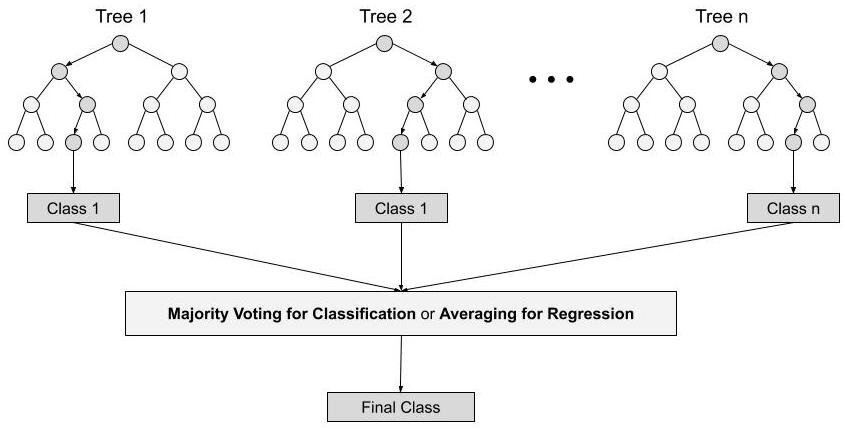
\includegraphics[width=\textwidth,height=\textheight,keepaspectratio]{Random_forest.jpg}
    \caption{Random Forest}
    \label{fig:Model}
\end{figure}


\subsubsection{Random Forest Regressor}
Random forest is an ensemble of decision trees. This is to say that many trees, constructed in a certain “random” way form a Random Forest. 

Each tree is created from a different sample of rows and at each node, a different sample of features is selected for splitting. 
Each of the trees makes its own individual prediction. 
These predictions are then averaged to produce a single result. 

\subsubsection{Extra Trees Regressor}
Extra Trees is a machine learning approach that combines the predictions of multiple decision trees into a single forecast.

It is a commonly used random forest algorithm. Although it uses a simpler approach to create the decision trees used as members of the ensemble, it can often yield similar or better results than the random forest algorithm.

Both the techniques discussed above are tree algorithms, with random forest regressor using resampling and the latter using only the original data to create the random forest.

\subsubsection{MultiOutput Regressor}
The above linear out put models are run more times to get multiple values to match with the target size, in this case to match with the 4 visual concepts.

\subsection{Deep Learning model}

\subsection{Training and Validation set}
As discussed in the above section, the random forest regressor brings in a concept of Bootstrap resamplaing bringing in new data that can diverge from actual data for training, and hence decreasing its training accuracy compared to the Extra trees regressor.
Whereas the validation accuracy of the random forest regressor faired better than Extra trees by approximately 0.01 %

\section{Tested Models}
We tested on the above stated training models, and additionally a DL model with the architecture as shown below. But the error value was too high, hence was discarded at the end.
 \ref{Model1Architecture}
\begin{center}
\begin{figure}[h]
    \centering
    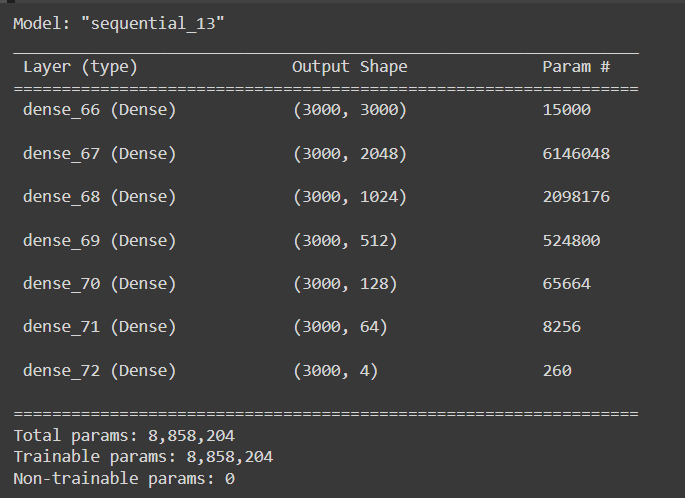
\includegraphics[width=\textwidth,height=\textheight,keepaspectratio]{DL_model.png}
    \caption{DL model}
    \label{fig:Randomforest}
\end{figure}
\end{center}

This followed the same pre-processing techniques from the proposed model. The average validation accuracy measured was only 0.15 .We suspect that lack of data can attributed to this poor accuracy. Hence we had to alter our model to a much simpler neural network that can work with smaller amount of data. 


\section{Hardware used}
Google Colab notebook was used to train the model. A general purpose RAM 
size of 8GB was alloted with a 2.3GHz Intel Xenon CPU.


\section {Code}
The resources used by JBTTM for CLEF aware, including the research papers, exploratory data analysis, and code can be found here: \url{https://github.com/AAnirudh07/CLEF-2022}

\section{Result}
The proposed models had an accuracy of 0.137 pearson correlation value , after submitting to the aicrowd submissions. 

\section{Conclusion}
 

\bibliographystyle{splncs}

%
\bibliography{references}

%
\end{document}
